\documentclass[twocolumn,a4paper]{article}
\usepackage{xcolor,
  graphicx,
  multicol,
  listings,savetrees}
\setlength\columnseprule{.5pt}
\setlength\columnsep{2em}
% \usepackage[a4paper,
%       scale={0.92,1.03},
%       includeheadfoot
%       ]{geometry}
\usepackage{palatino}
\definecolor{fontys}{rgb}{.3,0,.3}
\providecommand\Code[1]{{\color{fontys}\ttfamily#1}}
\lstset{language=Java,basicstyle={\ttfamily}}
\author{Pieter~van~den~Hombergh}
\title{Test driven development of a Stack}
\begin{document}
% \sloppy
\maketitle

\section*{Test Driven Develop Two Stacks.}

Derive the test from the requirements of the stack.
Use the design from the diagram.
\begin{figure}[htbp]
  \begin{center}
    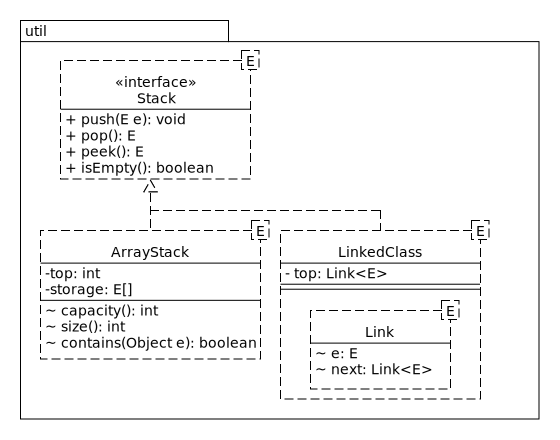
\includegraphics[width=\linewidth]{figures/twostacks}
    \caption{Stack design and alternative implementation classes}
  \end{center}
\end{figure}
When  implementing,  you create an array based stack first, called
\lstinline{ArrayStack<E>}. After that is complete, you create a
\lstinline{LinkedStack<E>}, starting from the same requirements and tests. Do you see a way to reuse code
(or test code) here? Hint: Think of a class hierarchy in the test
classes too. But first, start simple, then refactor.

\textbf{TDD}: Write your tests first. Derive them from the requirements given below.

\section*{Requirements of a Stack}

\begin{itemize}
\item The Stack should be generified, that is accept a Type parameter
  on instantiation as in  \lstinline{Stack<E>}.
\item An empty Stack reports \lstinline{isEmpty()} true.
\item When you \lstinline{push(x)} an element onto a stack, \lstinline{peek()} should return the
  \textit{same} object \lstinline{x}.
\item When you \lstinline{push(x)} an element onto a stack,
  \lstinline{pop()} should return the \textit{same} element
  \lstinline{x} and that element should no longer be on or in the stack.
\item When you push the elements from a \Code{list(a,b,c,d\ldots)} in this
  order onto a stack,
  and then \lstinline{pop()} the elements of that stack, the elements should come off in
  the reverse order.
\item For the implementations:
  \begin{description}
  \item[ArrayStack] An \Code{ArrayStack} should have the following
    additional package private methods. They are to be used in tests:
    \begin{itemize}
    \item An ArrayStack should be able to report it's
      current size (how many elements are stored).
    \item An ArrayStack should be able to report it's
      current capacity (how many elements can be stored).
    \item An ArrayStack has a method to check if an Object is contained,
      to verify that the requirement to actually erase the element on
      pop is implemented.
    \end{itemize}
  \item[LinkedStack] A linked stack has no extra requirements beyond
    the methods defined in the interface.
  \end{description}
\end{itemize}

\section*{Implementation hints}
Work test driven. Derive a test method (and its name) from the
requirements and code it in the same package as the Stack interface.

For instance, name your first test method \lstinline{public void a_new_stack_is_empty()}. 

\subsection*{Let the IDE do the work}
If your start with declaring the complete interface, you may be best
of by first implementing a \Code{DummyStackAdapter} that implements all
methods to satisfy the compiler and runtime. Simply accept what NetBeans IDE
generates for you, thrown exceptions and all. Then \textit{extend}
this \Code{DummyStackAdapter} with the class that you want to implement,
implementing the methods in ``natural'' order. When you are done with
all methods in both implementation, throw the \Code{DummyStackAdapter} away (it is
useless anyway, since all its methods are overwritten, right) and
modify the\\
\lstinline{extends DummyStackAdapter<E>} to\\ 
\lstinline{implements Stack<E>}.

\subsection*{Hints to ArrayStack}
\begin{itemize}
\item Internally use an array of Object.
\item Design the stack on paper using pen or pencil (pencil is best).
  Good names and types for the members are
  \lstinline{E [] storage;} for the array and \lstinline{int top;} for the
  member that knows where the top-most element is. Initialize the members
  properly, either in a constructor or initialize at declaration.
\item Do not move or copy the elements around on push or pop. 
  Just update your \Code{top} to
  do the administration. 
\item An initial capacity of 4 should do.
\item This stack may overflow its array, so before you push, make
  sure you have sufficient capacity. Use a separate method that does
  so, call it \Code{ensureCapacity()}.
\item There is no need to shrink the stack back again when elements are
  popped off.
\item When you pop an element off the stack, make sure it's place in the
  storage is overwritten with \Code{null} to prevent leaking memory.
\end{itemize}

\subsection*{LinkedStack hints}\sloppypar
Imagine the structure of the linked stack as a chain with links and each
link carrying an element.

\paragraph{Make a drawing with paper and pencil.} Draw a stack with
three elements stored in it. Scan it in or make a photo with your
smart phone or tablet and add the
result to the repository. A nice touch would be to trim the scan
file down to size and include it in the javadoc for the linked
stack.

\begin{itemize}
\item Use a static inner class called \Code{Link}. Give it a final
  field of type E, named e and a field next, which can hold a
  reference to another link.
\item The stack is empty when \lstinline{top == null}.
\item The chain ``hangs'' by its top.
\item Push
  creates a new link, adds the current top as next and assigns this new
  link to top.
\item Pop takes the element from the top element and assigns top.next
  to top.
\item Peek simply returns top.element.
\item The LinkedStack does not need a \lstinline{size()}, a
  \lstinline{capacity()} or \lstinline{contains(Object o)} method.
\end{itemize}
\end{document}
